\documentclass[a4paper]{article}    % define document layout
%\documentclass[draft]{article}     % use draft option in packages
%-----------------------------
% preamble
%-----------------------------
\usepackage[sumlimits,]{amsmath}    % math equations and formulas
\usepackage{amsfonts}
\usepackage[utf8]{inputenc}         % use UTF-8 encoding
\usepackage[english]{babel}         % use English language
\usepackage{graphicx}              % insert images
%\usepackage[draft]{graphicx}        % do not render figures
\usepackage{subcaption}             % multiple images in one figure
\usepackage{hyperref}               % hyperlinks
\usepackage{float}                  % floating objects (figures, tables)
\usepackage{geometry}               % page size and margins
\geometry{a4paper, margin=1in}      % margins
\usepackage{ragged2e}               % text alignment
\usepackage[table]{xcolor}          % change cell color in tables
%\usepackage{multirow}               % merge rows in table
%\usepackage[thinc]{esdiff}          % macros for derivatives
\usepackage{enumitem}

% MATLAB code
\usepackage{listings}
\usepackage{color} %red, green, blue, yellow, cyan, magenta, black, white
\usepackage{xcolor}

\graphicspath{                      % path for figures
    {../figures/} 
}

\definecolor{codegreen}{rgb}{0,0.6,0}
\definecolor{codegray}{rgb}{0.5,0.5,0.5}
\definecolor{codepurple}{rgb}{0.58,0,0.82}
\definecolor{backcolour}{rgb}{0.95,0.95,0.92}

\lstdefinestyle{mystyle}{
    backgroundcolor=\color{backcolour},   
    commentstyle=\color{codegreen},
    keywordstyle=\color{magenta},
    numberstyle=\tiny\color{codegray},
    stringstyle=\color{codepurple},
    basicstyle=\ttfamily\footnotesize,
    breakatwhitespace=false,         
    breaklines=true,                 
    captionpos=b,                    
    keepspaces=true,                 
    numbers=left,                    
    numbersep=5pt,                  
    showspaces=false,                
    showstringspaces=false,
    showtabs=false,                  
    tabsize=2
}
\lstset{style=mystyle}

%-----------------------------
% body
%-----------------------------
\begin{document}

\begin{figure}
    \centering
    % UNICAMP logo
    \begin{subfigure}{0.45\textwidth}
        \centering
        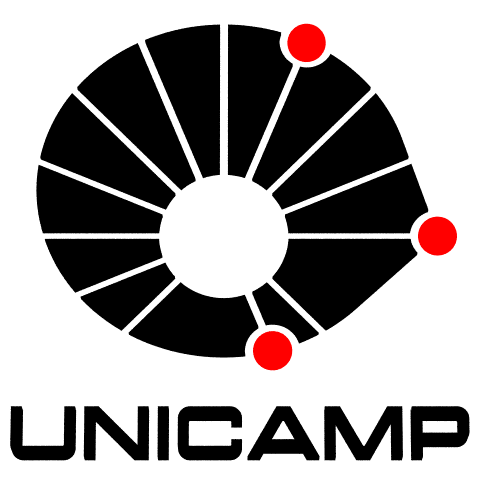
\includegraphics[width=1.5cm]{unicamp}
%        \label{fig:unicamp}
    \end{subfigure}
    \hfill
    % FEEC logo
    \begin{subfigure}{0.45\textwidth}
        \centering
        
\includegraphics[width=1.5cm]{feec}
%        \label{fig:feec}
    \end{subfigure}
\end{figure}

\title{
    \vspace{5cm}
    IA353A - Neural Networks\\
    EC2
    \vspace{1cm}
}
\author{
    Rafael Claro Ito\\
    (R.A.: 118430)
    \vspace{11cm}
}
%R.A.: 118430
%ito.rafael@gmail.com
\date{August 2020}
\maketitle
\newpage

\setcounter{section}{7}
%=================================================
\section*{Question 7}
%=================================================

%------------------------
\subsection{Transferência negativa}
%------------------------
\paragraph{Transferência negativa é quando tem-se uma piora de performance ao compartilhar informação de tarefas em MTL. Isso ocorre quando as tarefas envolvidas não são relacionadas. Ou seja, para ser possível trabalhar com \emph{multitask learning}, as tarefas envolvidas devem ter uma relação próxima.}

%------------------------
\subsection{Camadas compartilhadas}
%------------------------
\paragraph{Uma das estratégias usada em MTL consiste em incluir na função custo a ser otimizada as perdas de cada uma das tarefas envolvidas, por exemplo com uma soma ponderada (para o caso de as escalas da perdas serem diferentes). Assim, o ajuste dos pesos das camadas compartilhadas da arquitetura de MTL mostrada na figura \ref{fig:q7} consiste em apresentar para a rede padrões das tarefas consideradas, calcular o erro na saída da tarefa em questão e fazer o uso do \emph{backpropagation} normalmente para atualização dos pesos (se mini batches forem usados, misturar dados das tarefas para formar os mini batches pode ajudar no treinamento).}

\paragraph{Se treinarmos cada tarefa de aprendizado individualmente, na prática estamos ignorando informações das outras tarefas relacionadas que poderia ajudar ainda mais na métrica da tarefa em treinamento. Quando usamos todas essas informações, estamos compartilhando representações entre as tarefas relacionadas e isso faz com o que o modelo generalize melhor na tarefa original.}

\begin{figure}[H]
    \centering
    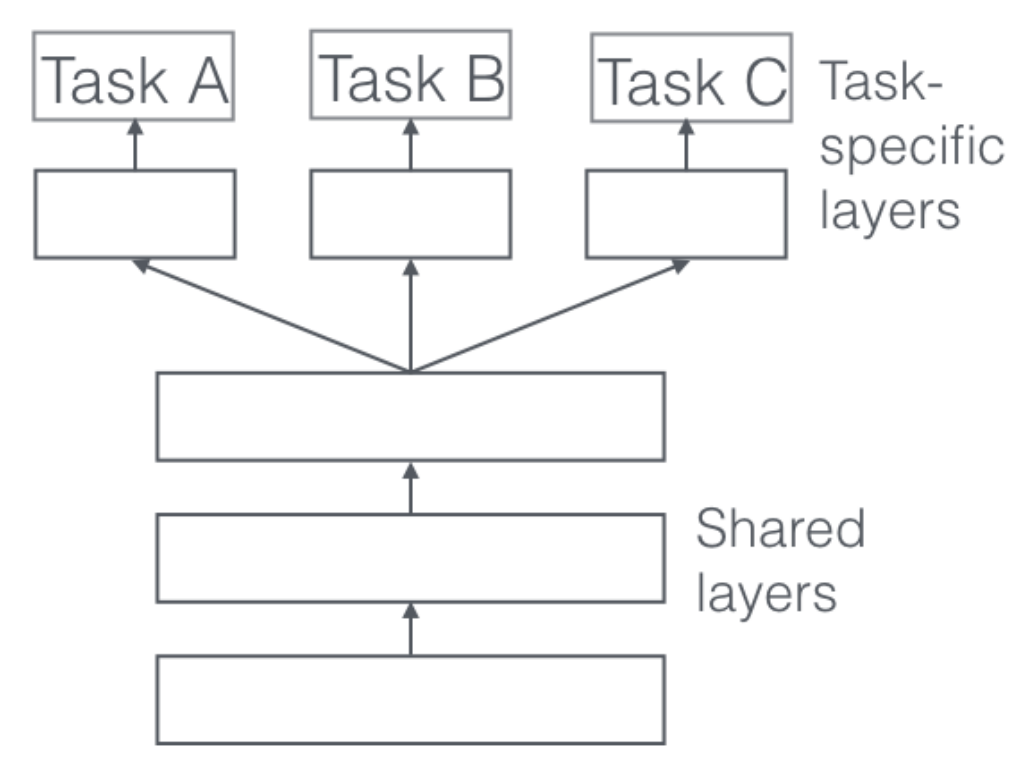
\includegraphics[width=6cm]{Q7}
    \caption{Abordagem de compartilhamentos de parâmetros \emph{Hard}}
    \label{fig:q7}
\end{figure}

\paragraph{De fato, esta é uma das vantagens em se usar MTL. Conforme citado no artigo \href{https://arxiv.org/pdf/1706.05098.pdf}{(Ruder, 2017)}, recomendando como leitura de apoio para a resposta desta questão, \href{https://link.springer.com/content/pdf/10.1023/A:1007327622663.pdf}{(Baxter, 1997)} mostra que o risco de \emph{overfitting} nos parâmetros das camadas compartilhadas é de ordem N (onde N é o número de tarefas) vezes menor do que o risco de \emph{overfitting } nas camadas de saída específicas para cada tarefa. E isso faz sentido, pois quanto mais tarefas considerarmos simultaneamente, mais o modelo precisa encontrar uma representação que capture todas as tarefas, e portanto menor é a chance de \emph{overfitting}.}

\paragraph{Uma outra forma de enxergar MTL, também recorrendo à leitura de apoio, é olhar para MTL como uma forma de transferência indutiva, que melhora o modelo introduzindo um \emph{bias} indutivo. Para o caso de MTL, esse \emph{bias} indutivo é fornecido pelas tarefas auxiliares, e isso faz com que o modelo dê preferência para hipóteses que explicam mais de uma tarefa, o que geralmente leva a soluções que generalizam melhor.}

\paragraph{Por fim, um último fato relevante a ser levantado é que mesmo que a função custo a ser otimizada seja apenas de uma tarefa, incluir tarefas auxiliares (que tenham alguma relação com a tarefa original) pode melhorar o desempenho na tarefa original, por conta de uma melhor representação dos dados nas camadas compartilhadas.}

%------------------------
\subsection{MALSAR}
%------------------------
\paragraph{Em machine learning, para problemas de regressão e classificação geralmente temos o seguinte problema de otimização para ser resolvido:}

\[\min_W \mathcal{L}(W) + \Omega(W)\]

\paragraph{Nesta equação, $W$ representa os parâmetros a serem ajustados a partir de dados durante a etapa de treinamento, $\mathcal{L}(W)$ representa a função de perda e $\Omega(W)$ o termo de regularização.}

\paragraph{No contexto de MTL, $W$ continua sendo os parâmetros ajustáveis. Entretanto, como estamos trabalhando com mais de uma tarefa, podemos ter um $W$ para cada tarefa, sendo que parte dos parâmetros de $W$ são compartilhados entre as tarefas (por exemplo como no caso da figura \ref{fig:q7} do item anterior). Assim, na função de perda $\mathcal{L}(W)$ devemos incorporar os erros associados a cada uma das tarefas, podendo ser uma soma ponderada, por exemplo. $\Omega(W)$ continua sendo o termo de regularização, mas que agora incorpora a relação entre as tarefas. Isto é, diferentes suposições a cerca do tipo de relações entre as tarefas leva a diferente termos de regularização.}

\paragraph{Em seguida, apresentaremos uma conformação possível para os termos de otimização da equação anterior:}

\[\min_W \sum_{i=1}^{t} ||W_i^T X_i - Y_i||_F^2 + \rho_1||W||_1\]

\paragraph{Essa formulação de MTL considera o método de regularização Lasso, que penaliza a norma $\ell_1$ de $W$. Esse tipo de regularização é tipicamente usado para introduzir esparsidade no modelo, forçando alguns parâmetros a zero e reduzindo a complexidade do modelo. Para a extensão da formulação de STL (\emph{Single-Task Learning}) para MTL temos que o parâmetro que controla a esparsidade é compartilhado entre todas as tarefas, assumindo assim que diferentes tarefas apresentam o mesmo parâmetro de esparsidade.}

\paragraph{Na equação anterior, temos:}
\begin{itemize}
    \item Função de perda: $\mathcal{L}(W) = \sum_{i=1}^{t} ||W_i^T X_i - Y_i||_F^2$
    \item Termo de regularização: $\Omega(W) = \rho_1||W||_1$
    \item Onde temos:
    \begin{itemize}
        \item $t$ é o número de tarefas consideradas
        \item $X_i$ e $Y_i$ são os dados de entrada e rótulos, respectivamente, para a tarefa $i$
        \item $\rho_1$ é o parâmetro de regularização que controla esparsidade
    \end{itemize}
\end{itemize}

\paragraph{O que foi apresentado vale para a regularização Lasso, podendo ser extendida para a regularização de quadrados mínimos alterando $\Omega(W)$ para $\rho_{L2}||W||_F^2$, ou ainda para elastic net somando este último termo ao apresentado para Lasso (ou seja, $\Omega(W) = \rho_1 ||W||_1 + \rho_{L2}||W||_F^2$).}

\newpage
%=================================================
\section*{Question 8}
%=================================================

\paragraph{Considerando a camada $q$ de uma rede neural MLP, temos:}
\[x^{[q]} = f(W^{[q]} x^{[q-1]} + b)\]

\paragraph{Onde:}
\begin{itemize}
    \item $x^{[q]}$ é a saída da camada $q$ após função de ativação;
    \item $W^{[q]}$ são os pesos dos neurônios da camada $q$;
    \item $x^{[q-1]}$ é a entrada da camada $q$ (saída da camada $q-1$);
    \item $f(\cdot)$ é a função de ativação da camada $q$;
\end{itemize}

\paragraph{Calculando a variância de ambos lados da equação anterior, temos:}

\[x^{[q]} = f(W^{[q]} x^{[q-1]} + b)\]
\[Var(x^{[q]}) = Var(f(W^{[q]} x^{[q-1]} + b))\]

\paragraph{Devemos agora fazer algumas considerações:}
\begin{enumerate}[label=(\roman*)]
    \item função de ativação $f(\cdot) = tanh$, sendo que no início do treinamento trabalha-se com os pesos próximos à região linear (próximo de zero), evitando neurônios operando na região de saturação e favorecendo o aprendizado nas primeiras iterações. Desta forma, considerando a região linear, podemos aproximar a função $tanh$ para uma função identidade;
    \item $W$ e $x$ são independentes entre si;
    \item $W$ é uma variável aleatória i.i.d. (independente e identicamente distribuída). Isso geralmente é verdade para a inicialização;
    \item $x$ é uma variável aleatória i.i.d. (independente e identicamente distribuída). Embora nem sempre isso seja verdade (por exemplo, pixels de uma imagem geralmente apresentam alta correlação entre pixels ao redor), faremos essa consideração;
\end{enumerate}

\paragraph{Continuando o desenvolvimento da equação anterior:}
\[Var(x^{[q]}) = Var(f(W^{[q]} x^{[q-1]} + b))\]

\paragraph{A partir de i), temos:}
\[Var(x^{[q]}) = Var(W^{[q]} x^{[q-1]} + b)\]

\paragraph{Se duas variáveis são independentes entre si, temos a igualdade:\\
\href{https://en.wikipedia.org/wiki/Variance\#Product_of_independent_variables}{https://en.wikipedia.org/wiki/Variance\#Product\_of\_independent\_variables}:}
\[Var(XY) = [\mathbb{E}(X)]^2 Var(Y) + [\mathbb{E}(Y)]^2 Var(X) + Var(X)Var(Y)\]

\paragraph{Vamos agora abrir o produto das matrizes $W$ e $x$ em uma soma dos produtos de seus termos  $w_i$ e $x_i$. Usando também a consideração dada por ii) e sabendo que $b$ é uma constante (e portanto sua variância é zero), temos que:}
\[Var(x^{[q]}) = Var(W^{[q]} x^{[q-1]} + b)\]
\[Var(x^{[q]}) = Var(\sum_{i=1}^{n^{[q-1]}} w_i^{[q]} x_i^{[q-1]})\]
\[Var(x^{[q]}) = \sum_{i=1}^{n^{[q-1]}} Var(w_i^{[q]} x_i^{[q-1]})\]
\[Var(x^{[q]}) = \sum_{i=1}^{n^{[q-1]}}[\mathbb{E}(w_i^{[q]})]^2 Var(x_i^{[q-1]}) + [\mathbb{E}(x_i^{[q-1]})]^2 Var(w_i^{[q]}) + Var(w_i^{[q]})Var(x_i^{[q-1])})\]

\paragraph{A partir de iii) e iv), temos que $\mathbb{E}(w_i) = 0$ e $\mathbb{E}(x_i) = 0$, sendo ambos $W$ e $x$ variáveis i.i.d. Assim:}
\[Var(x^{[q]}) = \sum_{i=1}^{n^{[q-1]}} Var(w_i^{[q]})Var(x_i^{[q-1]})\]
\[\boxed{Var(x^{[q]}) = n^{[q-1]} Var(w^{[q]})Var(x^{[q-1]})}\]

\paragraph{Queremos provar que $b = \sqrt{\frac{3}{n^{[q-1]}}}$ para que a variância da entrada da camada $q$ seja igual a variância da camada $q-1$.}

\paragraph{Sabendo que a variância de uma variável aleatória que segue uma distribuição uniforme entre $a$ e $b$, isto é, $X \sim \mathbb{U}[a,b]$, é dada por: $Var(X) = \frac{(b-a)^2}{12}$ (\href{https://proofwiki.org/wiki/Variance_of_Continuous_Uniform_Distribution}{prova}). Temos:}
\[Var(x^{[q]}) = n^{[q-1]} Var(w^{[q]})Var(x^{[q-1]})\]
\[Var(x^{[q]}) = n^{[q-1]} \cdot \frac{(b-(-b))^2}{12} \cdot Var(x^{[q-1]})\]
\[Var(x^{[q]}) = n^{[q-1]} \cdot \frac{(2b)^2}{12} \cdot Var(x^{[q-1]})\]
\[Var(x^{[q]}) = n^{[q-1]} \cdot \frac{4b^2}{12} \cdot Var(x^{[q-1]})\]

\paragraph{Como queremos $Var(x^{[q]}) = Var(x^{[q-1]})$, temos:}
\[n^{[q-1]} \cdot \frac{4b^2}{12} = 1\]
\[b^2 = \frac{12}{4 \cdot n^{[q-1]}}\]
\[\boxed{b = \sqrt{\frac{3}{n^{[q-1]}}}}\]

\newpage
\setcounter{section}{9}
\setcounter{subsection}{0}
%=================================================
\section*{Question 9}
%=================================================

%------------------------
\subsection{Principais seções do padrão de documentação}
%------------------------
\paragraph{As principais seções do padrão de documentação de datasets são mostradas na seção 3 do artigo, entitulada ``Questions and Workflow''. Os itens desta seção, assim como uma breve descrição são apresentados a seguir:}

\begin{itemize}
    \setlength\itemsep{0mm}
    \item \textbf{Motivação:} razões para a criação do dataset (propósito de tarefa específica, preenchimento de alguma lacuna na área), informações a cerca de quem ou qual grupo o criou, se houve alguma apoio ou financiamento para a construção do dataset.
    \item \textbf{Composição:} informações com respeito a composição do dataset, como por exemplo, do que se tratam os dados, se há rótulos e quais, quantidade de cada classe (se aplicável), divisão em treinamento/validação/teste recomendada, fontes de ruído nos dados, se os dados estão relacionados a pessoas, etc.
    \item \textbf{Processo de coleta:} informações sobre a construção do dataset permitindo outras pessoas reconstruí-lo (quando aplicável) sem ter acesso a ele. Aqui temos perguntas do tipo, se os dados foram coletados de algum sensor ou humanos, se os dados foram observados diretamente, que tipo de pessoa participou do processo de coleta dos dados e se elas foram compensadas, se há algum aspecto ético envolvido, etc.
    \item \textbf{Pré-processamento/limpeza/rotulamento:} descrição sobre o processamento e metodologia usada nos dados crus (fornecendo-os quando possível) e informação do software usado para isso quando aplicável.
    \item \textbf{Uso:} quais os casos de uso deste dataset, links para artigos que usufruem do dataset em questão, situações em que o dataset não deve ser usado.
    \item \textbf{Distribuição:} informações a respeito da distribuição dos dados. Se serão ou não distribuídos, onde e como serão (página web, GitHub, API, compactado), quando, qual a licença de uso, etc.
    \item \textbf{Manutenção:} por fim, informações a respeito de quem está hospedando os dados, quem está dando manutenção e suporte no dataset, contato do responsável, se há alguma errata, planos de atualização (o quê e quando), suporte a versões anteriores, entre outros.
\end{itemize}

\paragraph{Dois exemplos de datasheet para dataset são mostrados no apêndice do artigo. Um para o dataset ``Labeled Faces in the Wild'' e outro para o dataset  ``Pang and Lee’s polarity''.}

%------------------------
\subsection{Artigos com propósitos similares}
%------------------------

%------------------------
\subsubsection{Artigo 1}
%------------------------
O primeiro artigo é de um grupo da IBM Research e apresenta os FactSheets. Assim como os datasheets de componentes inspiraram o artigo usado como base desta questão, os SDoCs (supplier’s declarations of conformity) foram usados como base neste artigo de 2018 para propor os FactSheets.

\begin{itemize}
    \setlength\itemsep{0mm}
    \item título: FactSheets:  Increasing Trust in AI Servicesthrough Supplier’s Declarations of Conformity
    \item ano: 2018
    \item authors: Arnold et al. (IBM Research)
    \item arXiv: \href{https://arxiv.org/pdf/1808.07261.pdf}{https://arxiv.org/pdf/1808.07261.pdf}
\end{itemize}

%------------------------
\subsubsection{Artigo 2}
%------------------------
O segundo artigo também é de 2018 de um grupo da Google e apresenta os Model Cards. Um dos autores do artigo é o autor principal do artigo ``Datasheets for Datasets'' (Timnit Gebru), usado como base para esta questão. O artigo propõe um padrão de relatório para \textbf{modelos} treinados de machine learning, apresentando exemplos para dois modelos.

\begin{itemize}
    \setlength\itemsep{0mm}
    \item título: Model Cards for Model Reporting
    \item ano: 2018
    \item authors: Mitchell et al. (Google)
    \item arXiv: \href{https://arxiv.org/pdf/1810.03993.pdf}{https://arxiv.org/pdf/1810.03993.pdf}
\end{itemize}

\newpage
\setcounter{section}{10}
\setcounter{subsection}{0}
%=================================================
\section*{Question 10}
%=================================================

%------------------------
\subsection{EfficientNet}
%------------------------
\paragraph{O artigo \href{https://arxiv.org/pdf/1905.11946.pdf}{(Tan \& Le, 2019)} propõe uma forma de escalar modelos baseados em redes convolucionais (ConvNets), como por exemplo MobileNets e ResNet, levando em conta três parâmetros avaliados conjuntamente: profundidade, largura e resolução. Adicionalmente, os autores usam um método de NAS (\emph{neural architecture search}) para encontrar um modelo base (baseline), para em seguida usar o método de escalamento proposto e obter uma família de modelos denominada \emph{EfficientNets}, cujos resultados são impressionantes, sendo mais eficientes em termos de custo computacional (modelos menores e mais rápidos) e performance, com resultados melhores atingindo o estado da arte (SOTA) para base de dados como ImageNet, CIFAR-100 e outras.}

\paragraph{Supondo que se queira um modelo maior que use $2^N$ mais recursos, propõe-se aumentar a rede multiplicando os três parâmetros pelas seguintes constantes: profundidade multiplicada por $\alpha^N$, largura multiplicada por $\beta^N$ e tamanho da imagem (resolução) por $\gamma^N$, onde $\alpha$, $\beta$ e $\gamma$ são determinados através de um grid search no modelo original.}

\paragraph{Na seção 3 do artigo, os autores mostram que o escalamento dos três parâmetros aumentam a performance dos modelos, mas cada um seguindo sua própria curva de saturação (figura 3 do artigo). Assim, eles chegam na primeira observação. A segunda observação foi obtida através dos experimentos cujos resultados são mostrados na figura 4 do artigo. Aqui é concluído que para uma melhor acurácia e eficiência, é necessário um balanceamento entre os fatores de escala de largura, profundidade e resolução.}

\paragraph{O método de escalamento proposto é mostrado a seguir:}
\begin{itemize}
    \item profundidade: $d = \alpha^\phi$
    \item largura: $w = \beta^\phi$
    \item resolução: $r = \gamma^\phi$
\end{itemize}
\paragraph{Sujeito a:}
\begin{itemize}
    \item $\alpha \cdot \beta^2 \cdot \gamma^2 \approx 2$
    \item $\alpha \geq 1$
    \item $\beta \geq 1$
    \item $\gamma \geq 1$
\end{itemize}

\paragraph{O modelo base, denominado EfficientNet, foi obtido através de uma busca (NAS) multi-objetiva, procurando otimizar tanto a acurácia quanto FLOPS (operações de ponto flutuante por segundo). A função objetivo é dada por: $ACC(m) \times [FLOPS(m)/T]^w$, onde $ACC(m)$ e $FLOPS(m)$ é a acurária e FLOPS do modelo $m$, $T$ é o FLOPS alvo e $w$ controla o \emph{tradeoff} entre acurária e FLOPS. Tomando $w = -0.07$, chega-se no modelo EfficientNet-B0.}

\paragraph{A partir do modelo EfficientNet-B0, toma-se $\phi=1$ (dobro de recursos) e busca-se as constantes através de um \emph{grid search}. Encontra-se $\alpha=1.2$, $\beta=1.1$ e $\gamma=1.15$, satisfazendo a restrição $\alpha \cdot \beta^2 \cdot \gamma^2 \approx 2$. Em seguida, essas constantes são usadas para escalar diferentes modelos alterando o valor de $\phi$, obtendo-se os modelos EfficientNet-B1 até B7. Além destes modelos, MobileNets e ResNets também foram escaladas seguindo essa regra.}

\paragraph{A partir da seção 5 do artigo, são descritos os experimentos e resultados, discussões e conclusão. Conforme descrito no início da resposta desta questão, os resultados obtidos são impressionantes, ganhando tanto em performance (custo computacional) quanto em desempenho (acurária), atingindo um novo SOTA na área de visão computacional e ConvNets.}

%------------------------
\subsection{FixEfficientNet}
%------------------------
\paragraph{O segundo artigo \href{https://arxiv.org/pdf/2003.08237.pdf}{(Touvron et al., 2020)} é na verdade uma nota que complementa o artigo ``\href{https://arxiv.org/pdf/1906.06423.pdf}{Fixing the train-test resolution discrepancy}'', que introduz o método denominado FixRes.}

\paragraph{O artigo original mostra que as técnicas de \emph{data-augmentation} usadas até então induziam uma discrepância entre o tamanhos dos objetos visto pelo classificador durante o treinamento e durante a fase de teste. Assim, os autores propõe uma estratégia que otimiza a performance do classificador, empregando diferentes resoluções em teste e treinamento. Isso é feito através de um \emph{fine-tuning} da rede na resolução de teste.}

\paragraph{A nota que complementa o artigo original toma as diversas redes renomadas, dentre elas as EfficientNets do item anterior, e aplica o método FixRes para obter uma família de redes denominadas FixEfficientNet. Os resultados podem ser vistos na figura \ref{fig:q10}.}

\begin{figure}[H]
    \centering
    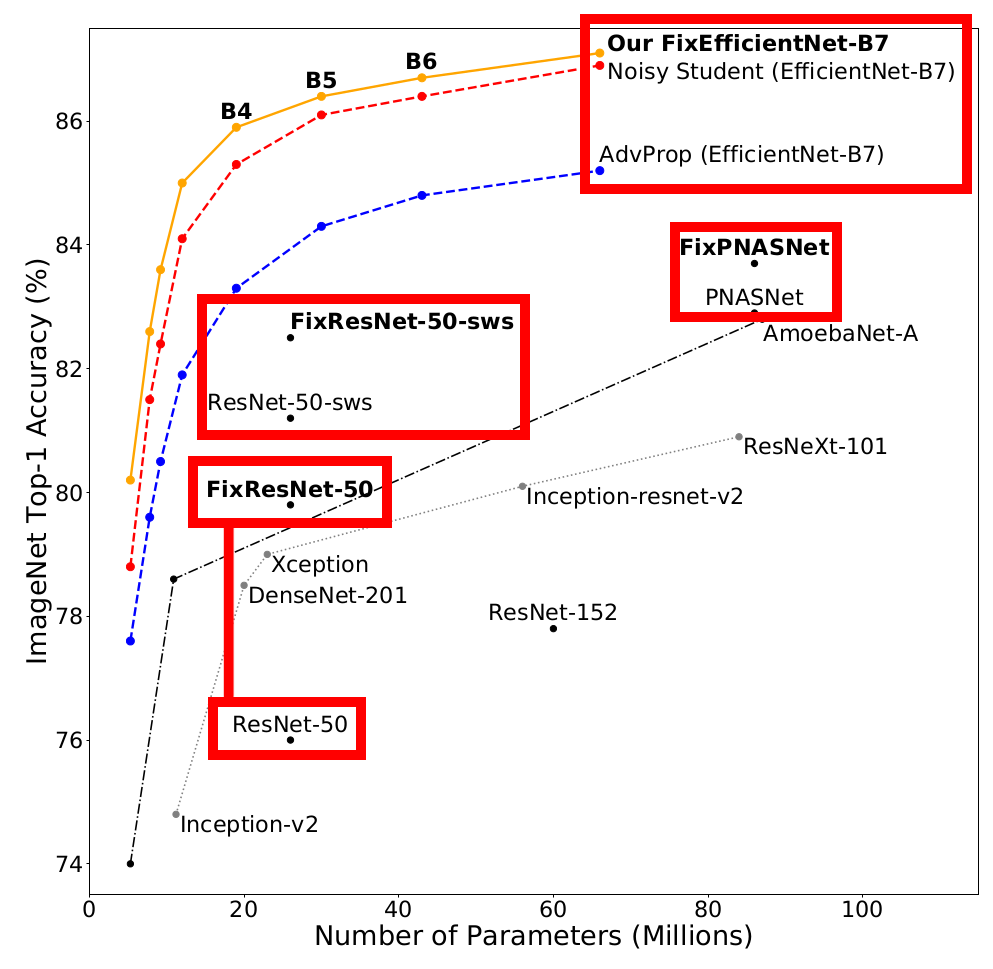
\includegraphics[width=10cm]{Q10_FixEfficientNet}
    \caption{Comparação entre diversas redes com e sem a aplicação do método FixRes}
    \label{fig:q10}
\end{figure}

\paragraph{Como podemos ver, em um curto período de tempo temos novos modelos SOTA. Alguns podem vir de arquiteturas novas (ex: EfficientNet em ConvNets e Transformers em NLP), outros de melhorias feitas na metodologia a partir de modelos já existentes (ex: escalamento apresentado no artigo da EfficientNet e método FixRes).}

%=================================================

\end{document}
